\chapter{Heterogeneous parallel ensembles: Combining strong learners\label{Ch03}}
In this chapter, we continue exploring parallel ensemble methods, but this time
focusing on \important{heterogeneous ensembles}. Heterogeneous ensemble methods use different
base-learning algorithms to directly ensure ensemble diversity.

Heterogeneous ensembles come in two
flavors, depending on how they combine individual base-estimator predictions into a
final prediction:
\begin{itemize}
    \item  \important{Weighting} methods—These methods assign individual base-estimator predictions
          a weight that corresponds to their strength. Better base estimators are assigned
          higher weights and influence the overall final prediction more. The predictions of individual base estimators are fed into a predetermined combination function, which makes the final predictions.
    \item \important{Meta-learning} methods—These methods use a learning algorithm to combine the
          predictions of base estimators; the predictions of individual base estimators are
          treated as metadata and passed to a second-level meta-learner, which is trained
          to make final predictions.
\end{itemize}

\figures{fig3-1}{
    Homogeneous
    ensembles (\autoref{Ch02}), such as bagging and random forests, use the same learning algorithm to train base estimators, and they achieve ensemble diversity through random sampling. Heterogeneous ensembles (this chapter) use different learning algorithms to achieve ensemble diversity.
}
\section{Fitting base estimators}
Unlike homogeneous ensembles, we can use any number of different learning algorithms and parameter settings to train base estimators. The key is to ensure that we choose learning algorithms that are
different enough to produce a diverse collection of estimators. The more diverse our
set of base estimators, the better the resulting ensemble will be.

\subsection{Individual predictions of base estimators}
\begin{tcolorbox}[title=Note]
    Most classifiers in scikit-learn can return the probability of a label rather than the
    label directly. Some of them, such as SVC, should be explicitly told to do so (notice
    that we set probability=True when initializing SVC), while others are natural
    probabilistic classifiers and can represent and reason over class probabilities. These
    probabilities represent each base estimator’s confidence in its prediction.
\end{tcolorbox}

Prediction probabilities are often called soft predictions. Soft predictions can
be converted to hard (0–1) predictions by simply picking the class label with the highest probability.

Of course, the most important step is how we
combine these individual predictions: by weighting or by meta-learning.

\begin{tcolorbox}[title=CAUTION]
    The prediction function just discussed is specifically written for two-
    class, that is, binary classification, problems. It can be extended to multiclass
    problems if care is taken to store the prediction probabilities for each class.
    That is, for multiclass problems, you’ll need to store the individual prediction
    probabilities in an array of size \verb|n_samples * n_estimators * n_classes|.
\end{tcolorbox}

\section{Combining predictions by weighting}
We should do in a manner consistent with the intuition, such that the final prediction is influenced more by the
stronger classifiers and less by the weaker classifiers.
\figures{fig3-7}{
    Each base classifier is assigned an importance weight that reflects how much
    its opinion contributes to the final decision. Weighted decisions of each base classifier
    are combined using a combination function.
}

\subsection{Majority vote}
Majority voting can be viewed as a weighted combination scheme in which each
base estimator is assigned an equal weight; that is, if we have $m$ base estimators,
each base estimator has a weight of $w_{clf}=\frac{1}{m}$
. The (weighted) predictions of the individual base estimators are combined using the majority vote.

\subsection{Accuracy weighting}
\subsubsection*{ACCURACY WEIGHTS USING A VALIDATION SET}

Once we’ve trained each base classifier (clf), we evaluate its performance on a validation set. Let $\alpha_t$ be the validation accuracy of the $t$-th classifier, $H_t$. The weight of each
base classifier is then computed as follows:
\begin{equation}
    w_t=\frac{\alpha_t}{\sum_{t=1}^m\alpha_t}
\end{equation}

Given a new example to predict $\bm{x}$, we can get the predictions of the individual classifiers, $y_t$. Now, the final prediction can be computed
as a weighted sum of the individual predictions:
\begin{equation}
    y_{final} = w_1y_1+w_2y_2+\cdots+w_m*y_m=\sum_{t=1}^{m}w_ty_t
\end{equation}

\begin{figure}
    \centering
    \begin{subfigure}[b]{.45\textwidth}
        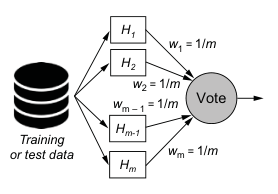
\includegraphics[width=\textwidth]{../Figures/fig3-8.png}
        \caption{Combining by majority voting. Bagging can be viewed as a simple weighting method applied to a homogeneous ensemble. All classifiers have equal weights, and the combination function is the majority vote. We can adopt the majority voting strategy for heterogeneous ensembles as well.}
    \end{subfigure}
    \hfill
    \begin{subfigure}[b]{.45\textwidth}
        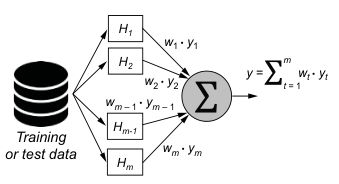
\includegraphics[width=\textwidth]{../Figures/fig3-9.png}
        \caption{Combining by performance weighting. Each classifier is assigned a weight proportional to its accuracy. The final prediction is computed as a weighted combination of the individual predictions.}
    \end{subfigure}
    \caption{Combining predictions by weighting}
\end{figure}

\subsection{Entropy weighting}

The entropy weighting approach is another performance-based weighting approach,
except that it uses entropy as the evaluation metric to judge the value of each base
estimator. Entropy is a measure of uncertainty or impurity in a set; a more disorderly
set will have higher entropy.

\begin{tcolorbox}[title=Entropy]
    Entropy, or information entropy to be precise, was originally devised by Claude Shan-
    non to quantify the “amount of information” conveyed by a variable. This is deter-
    mined by two factors: (1) the number of distinct values the variable can take, and (2)
    the uncertainty associated with each value.

    Entropy quantifies this notion of uncertainty across various outcomes. Entropy-based
    measures are commonly used during decision-tree learning to greedily identify the
    best variables to split on and are used as loss functions in deep neural networks.
\end{tcolorbox}

\subsubsection*{ENTROPY WEIGHTING WITH A VALIDATION SET}
Let $E_t$ be the validation entropy of the $t$-th classifier, $H_t$. The weight of each base classifier is
\begin{equation}
    w_t=\frac{\frac{1}{E_t}}{\sum_{t=1}^{m}\frac{1}{E_t}}
\end{equation}
There are two key differences between entropy weighting and accuracy weighting:
\begin{itemize}
    \item The accuracy of a base classifier is computed using both the true labels ytrue
          and the predicted labels ypred. In this manner, the accuracy metric measures
          how well a classifier performs. A classifier with high accuracy is better.
    \item The entropy of a base classifier is computed using only the predicted labels
          ypred, and the entropy metric measures how uncertain a classifier is about its
          predictions. A classifier with low entropy (uncertainty) is better. Thus, individual base classifier weights are inversely proportional to their corresponding
          entropies.
\end{itemize}

\subsection{Dempster-Shafer combination}
\subsubsection{DST FOR LABEL FUSION}
ST uses a number between 0 and 1 to indicate belief in a proposition, such as
“the test example x belongs to Class 1.” This number is known as a basic probability
assignment (BPA) and expresses the certainty that the text example $\bm{x}$ belongs to Class
1. BPA values closer to 1 characterize decisions made with more certainty. The BPA
allows us to translate an estimator’s confidence into a belief about the true label.

We’ve seen four methods of combining predictions into one final prediction. Three
use the predictions directly, while one use prediction probabilities. We can visualize the
decision boundaries produced by these weighting methods, as shown in \autoref{fig3-10}.
\begin{figure}
    \centering
    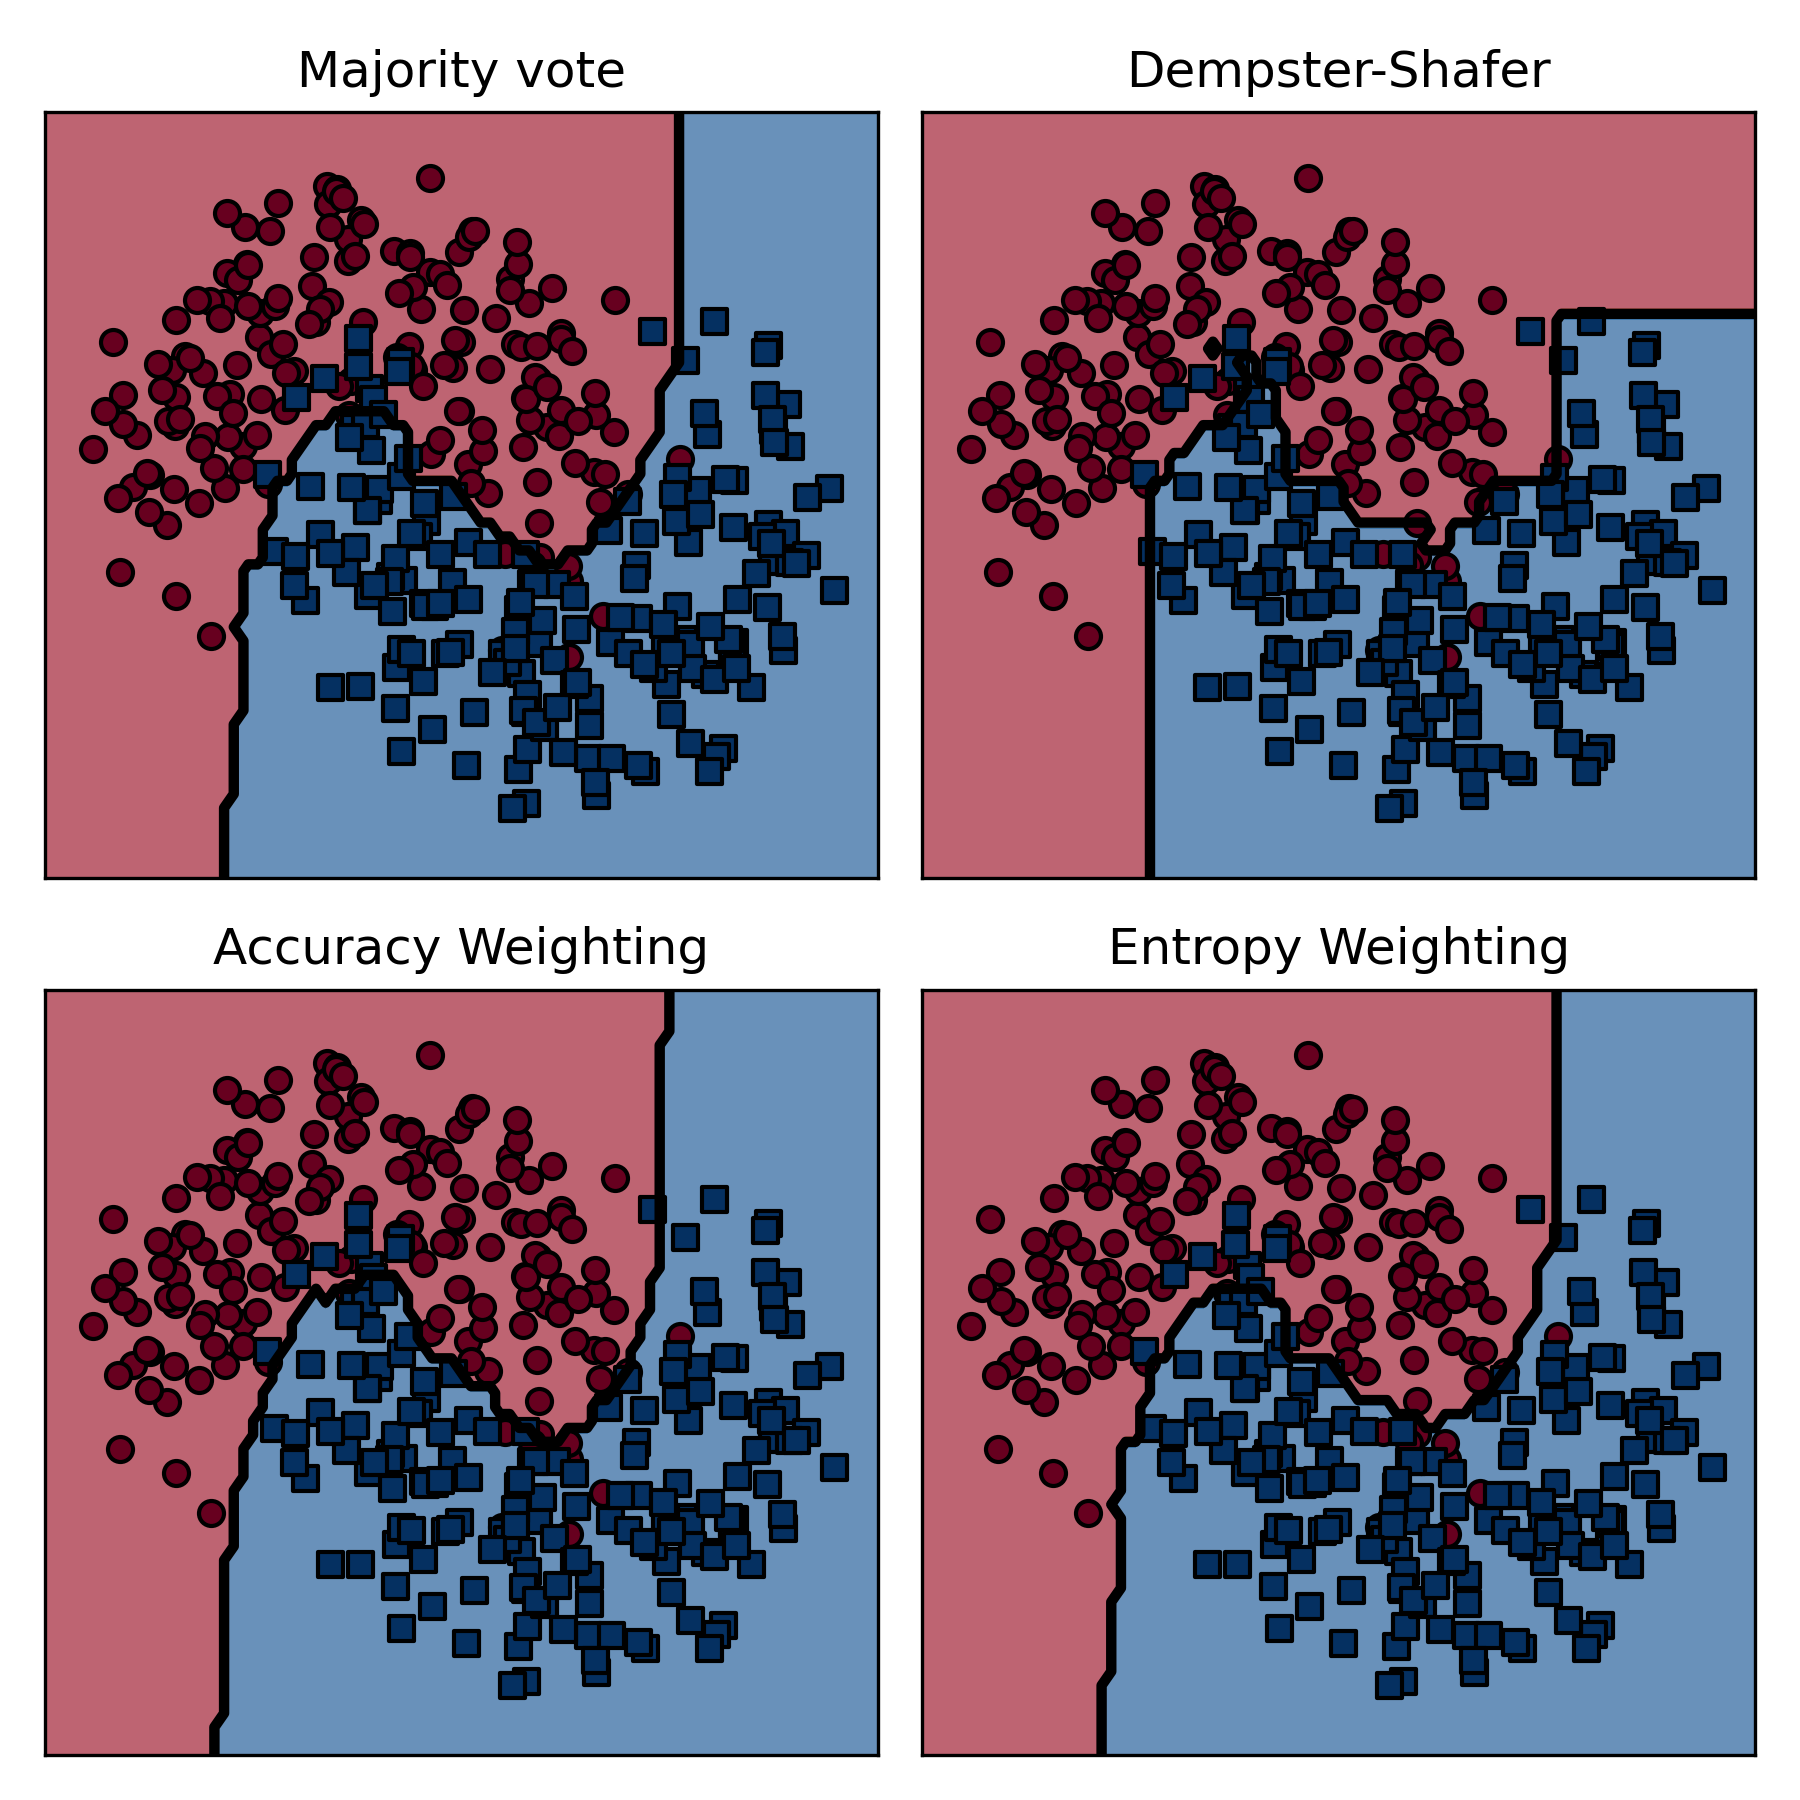
\includegraphics{../Figures/fig3-10.png}
    \caption{Decision boundaries of different weighting methods}
    \label{fig3-10}
\end{figure}